\chapter{Results and Validation}
\label{ch:Results_and_Validation}

This chapter presents the results of verification tests conducted on the Control Board (CB). The primary objective is to analyze the system’s feedback signals and compare them to the expected reference values. This comparison assesses whether the hardware and application software operate correctly and reliably.

\section{Current Sense Verification Results}
\label{sec:Results_and_Validation:CurrentSenseVerificationResults}

The Current Sense Verification evaluates the accuracy and consistency of the current measurement path on the Control Board. This evaluation involves analyzing digital feedback from the current-sensing circuit during both static and dynamic input tests. Reference values are transmitted to the \acs{DAC}, and feedback from the \acs{CB} is collected. The results are processed and plotted in MATLAB to verify that the outputs align with expectations. The following sections present the results from the static and dynamic tests.

\subsection{Static Test Results}
\label{sec:Results_and_Validation:CurrentSenseVerificationResults_static}

The Current Sense Static Verification assesses the sensing system's performance under constant input conditions. The feedback from the \acs{CB} is provided as a 12-bit digital value, while the reference values sent to the \acs{DAC} are 16-bit. MATLAB is utilized to scale, analyze, and verify these values.

During the static test, six distinct 16-bit values (0x0000, 0x3333, 0x6666, 0x9999, 0xCCCC, and 0xFFFF) were sequentially transmitted to the \acs{DAC}, each establishing a fixed current reference. The corresponding 12-bit digital feedback from the \acs{CB} was recorded for each value. These results were plotted in MATLAB to illustrate the relationship between the measured outputs and the reference values. As shown in Figure \ref{fig:Results:CurrentSense_Static}, the results exhibit a linear trend from 0x000 to 0xFFF, demonstrating that the current-sensing path performs as expected across various static inputs.

\begin{figure}[t]
	\centering
	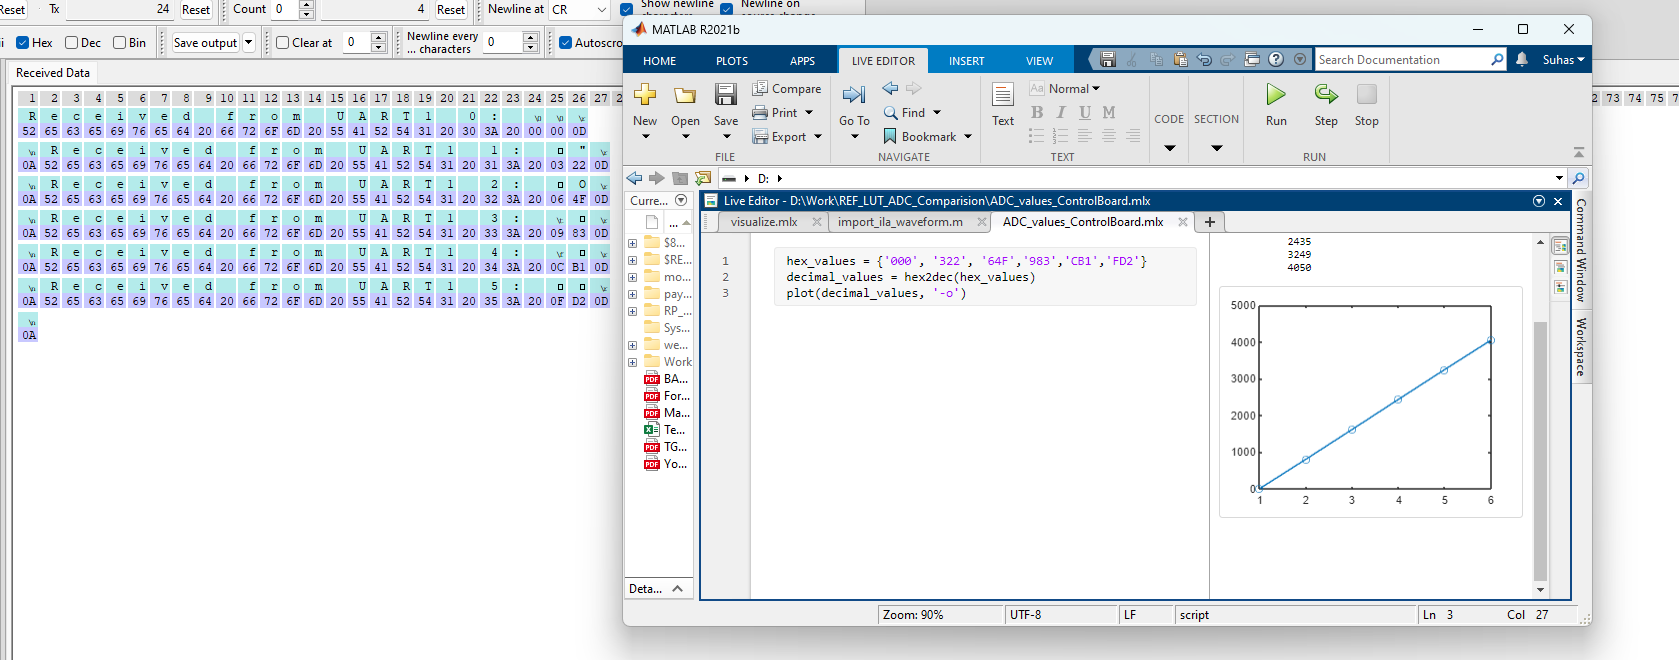
\includegraphics[width=0.90\textwidth, height=0.3\textheight]{gfx/diagrams/Static_Data_TEST.png}
	\caption{Current Sense Static Verification Results}
	\label{fig:Results:CurrentSense_Static}
\end{figure}

\subsection{Dynamic Test Results}
\label{sec:Results_and_Validation:CurrentSenseVerificationResults_dynamic}

This test evaluates the current-sensing chain's response to dynamic changes by comparing the frequency and waveform of feedback from the \acs{CB}. The \acs{CB} transmits sampled feedback to the Enclustra module through a 4096-byte \acs{FIFO}, with each 8-bit word representing a segment of a measurement. These 4096 bytes contain 2048 distinct 12-bit measurement values, transmitted in a packed format with least- and most-significant bytes for each sample.

\begin{figure}[H]
	\centering
	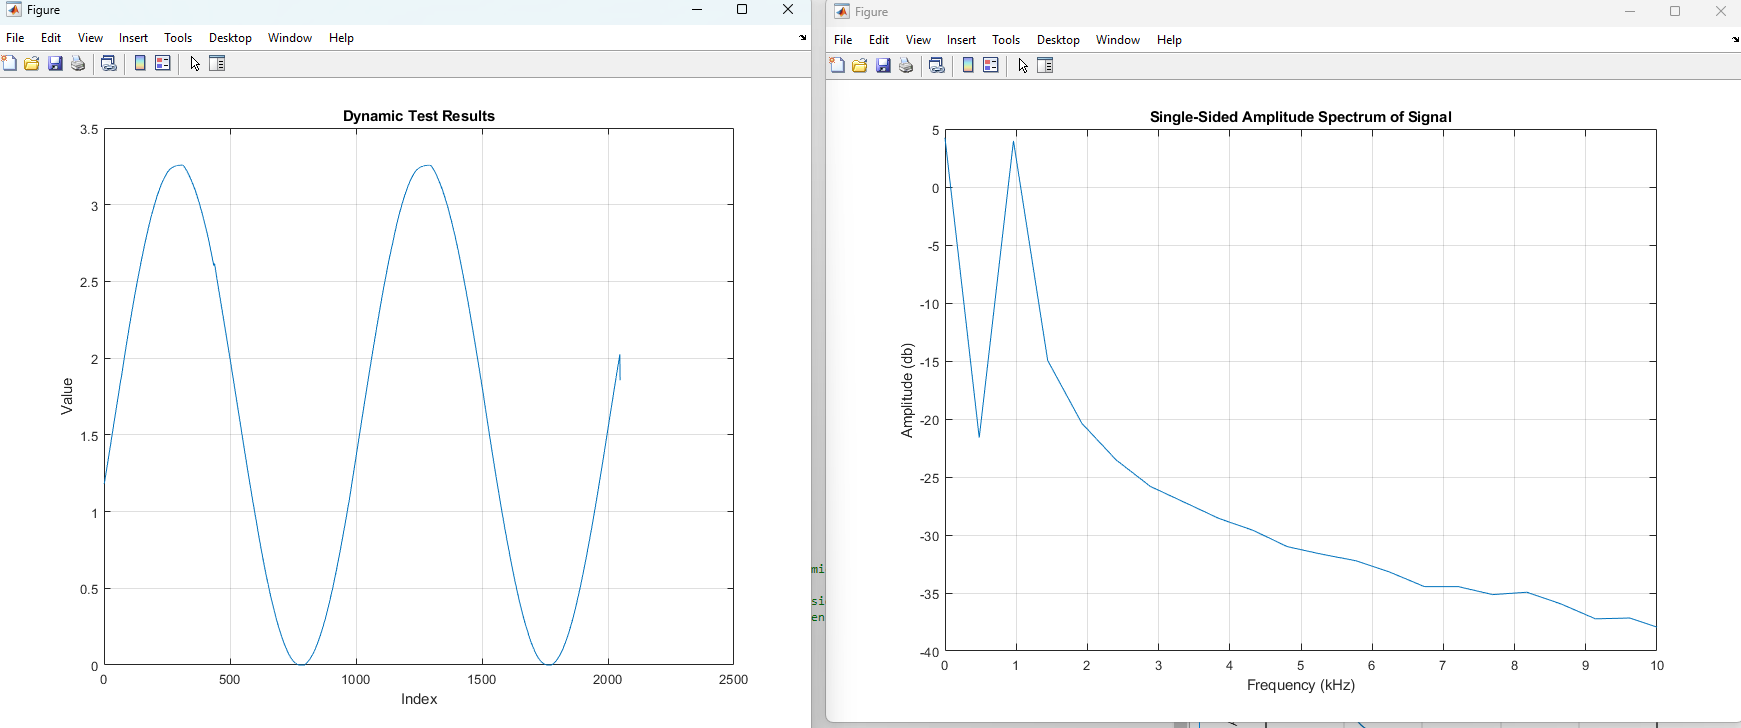
\includegraphics[width=0.90\textwidth, height=0.3\textheight]{gfx/diagrams/Dynamic_Result.png}
	\caption{Reconstructed time domain representation and \acs{FFT} of the feedback signal in matlab}
	\label{fig:Results:CurrentSense_dynamic}
\end{figure}

Upon receipt, the \acs{PS} analyses by applying \acs{FFT} and error values are calculated relative to the reference signal as mentioned in the section \ref{sec:Implementation:signal_Acquistion}. The accompanying figure \ref{fig:Results:CurrentSense_dynamic} presents the time-domain reconstruction of the received waveform, generated in MATLAB. The results demonstrate that the \acs{CB} accurately captures the dynamic current waveform and that the Enclustra \acs{PS} preserves the essential frequency content required for correct system operation.

\subsection{Reference Values vs measured Values}

The figure \ref{fig:Results:Static_Test_Comparision} compares the converted voltage values of the reference signal with those from the \acs{CB} during the static test. Digital values were converted to voltage using the method described in Section \ref{sec:Implementation:signal_Acquistion}. The plot demonstrates that the \acs{CB} feedback closely matches the reference signal, with sample points aligning as anticipated. These results confirm that the current sensing path accurately reproduces the static input across the tested range.

\begin{figure}[H]
	\centering
	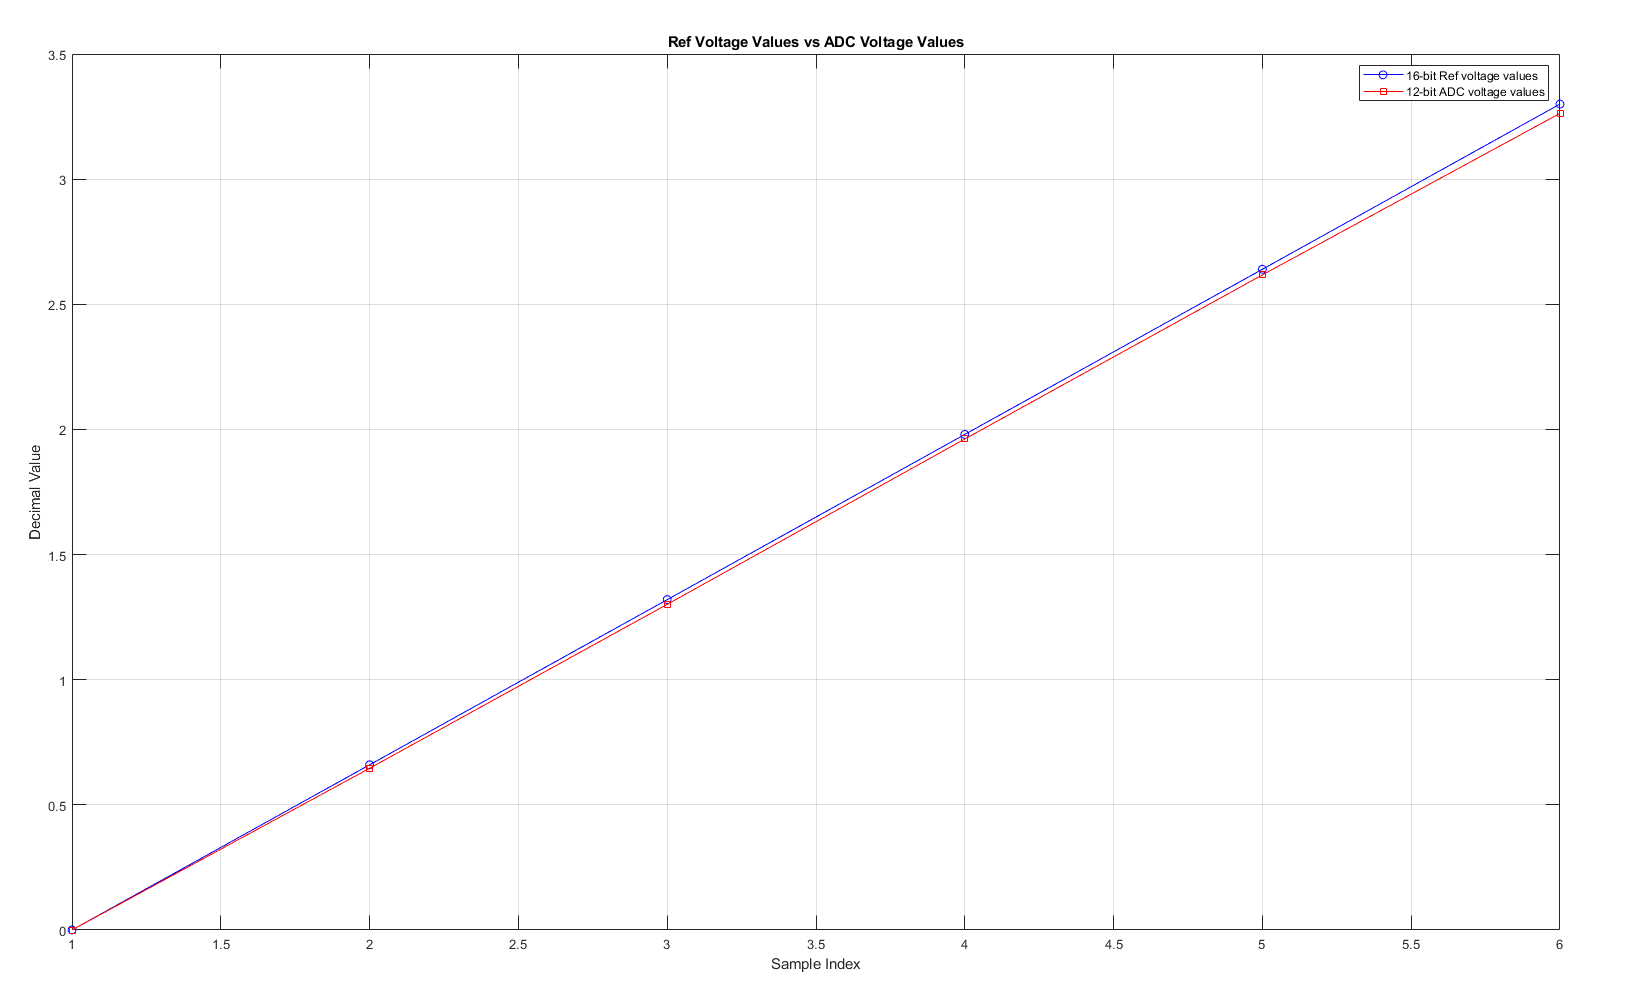
\includegraphics[width=0.80\textwidth, height=0.3\textheight]{gfx/diagrams/Static_Test_Comparision.png}
	\caption{Static Reference Voltage Values VS \acs{CB} feedback Voltage Values}
	\label{fig:Results:Static_Test_Comparision}
\end{figure}

Upon completion of the Current Sense Dynamic Verification, the frequency obtained from the \acs{CB} feedback and the associated error calculations relative to the reference signal are recorded in an output file to ensure documentation and traceability. The analysis results are presented in the accompanying figure \ref{fig:Results:Dynamic_Test_comparision}. When applying a 5\% error threshold, all calculated metrics, including the derived frequency, remain within acceptable limits. Consequently, the verification concludes with a “TEST PASSED” status, as indicated in the figure \ref{fig:Results:Dynamic_Test_comparision}, thereby confirming that the dynamic response of the sensing path satisfies the specified performance criteria.

\begin{figure}[t]
	\centering
	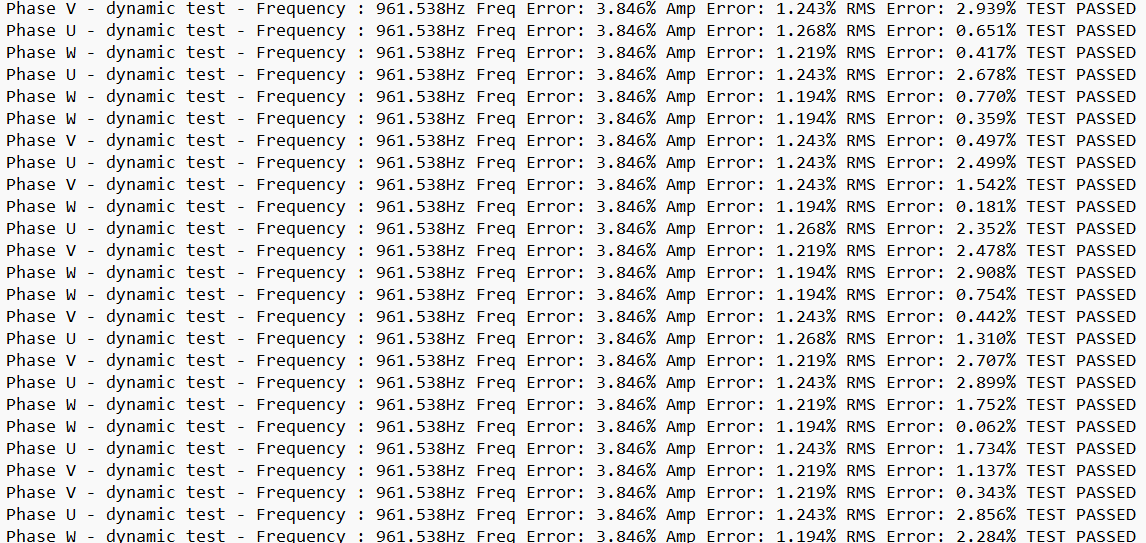
\includegraphics[width=0.85\textwidth]{gfx/diagrams/Current_Sense_perfect_results.png}
	\caption{Current Sense Dynamic Test Results}
	\label{fig:Results:Dynamic_Test_comparision}
\end{figure}

\begin{figure}[H]
	\centering
	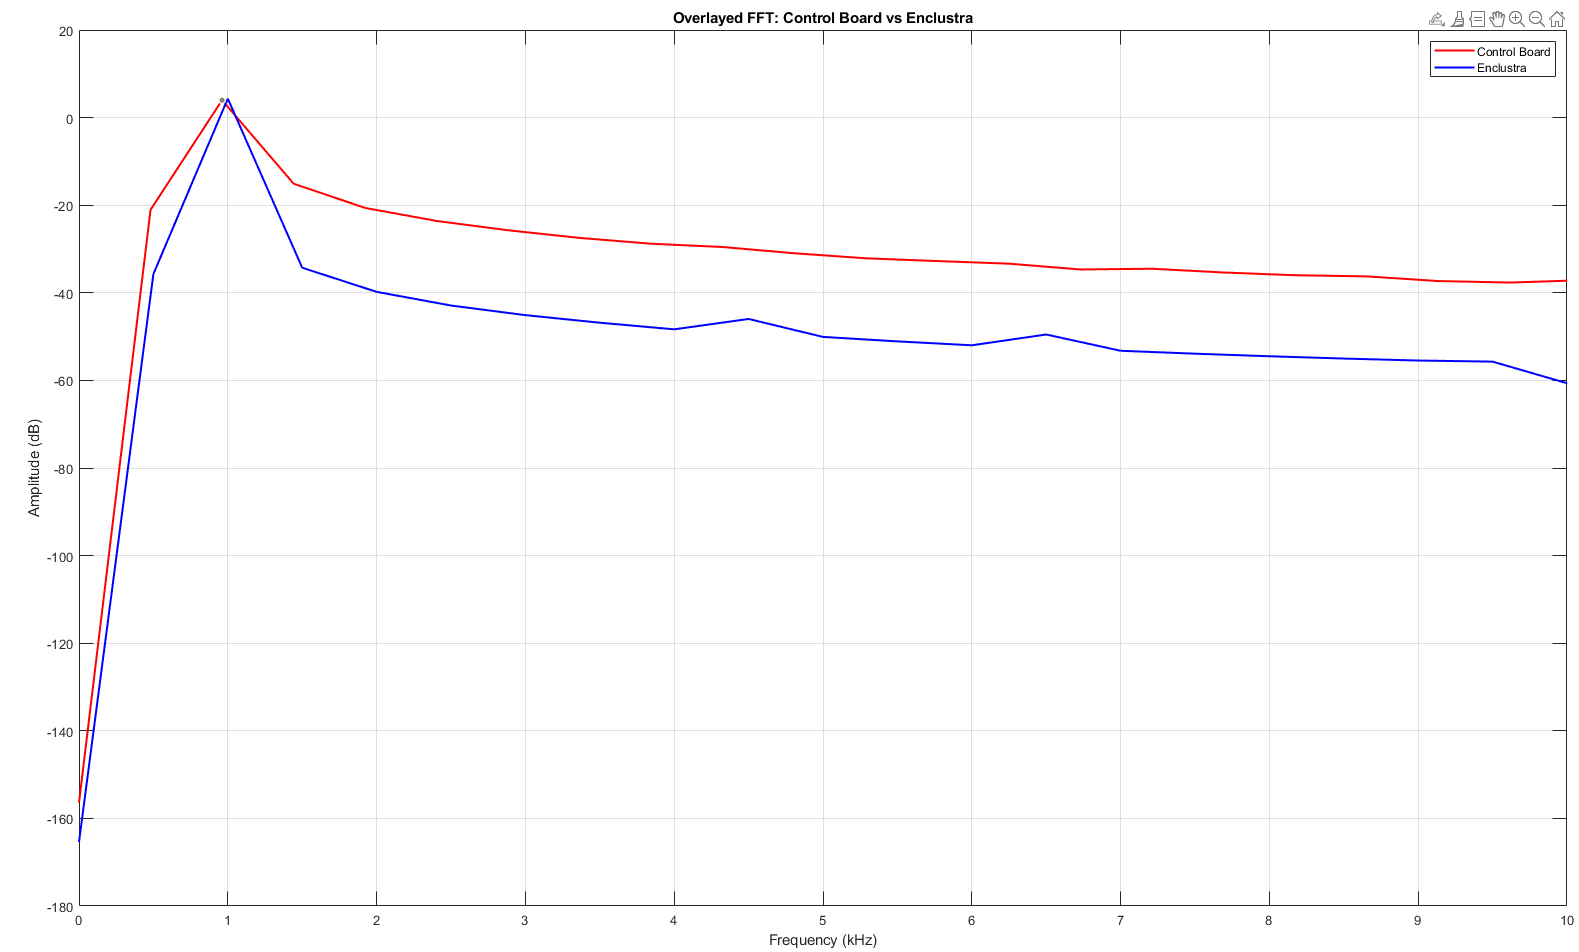
\includegraphics[width=0.80\textwidth]{gfx/diagrams/Overlayed_FFT_Dynamic.png}
	\caption{\acs{FFT} comparison of the reference 1 kHz digital signal and the feedback received from the Control Board.}
	\label{fig:Results:Overlayed_FFT_Comparision}
\end{figure}

The FFTs of both the \acs{CB} feedback signal and the original 1 kHz digital reference signal were calculated and analyzed in MATLAB. The resulting spectra are presented in the accompanying figure \ref{fig:Results:Overlayed_FFT_Comparision}. This MATLAB analysis corroborates the frequency characteristics observed in the experimental results, thereby supporting the validity and reliability of the Dynamic Current Sense Verification. The close correspondence between the reference spectrum and the measured feedback spectrum demonstrates that the sensing path maintains the expected dynamic behavior.

\section{\acs{PWM} Verification results}

The figure \ref{fig:Results:PWM_Results} presents a portion of the \acs{PWM} verification results. During this process, the \acs{PWM} frequency and duty cycle are transmitted to the \acs{CB}, which generates the corresponding \acs{PWM} signals and returns them to the verification platform. The \acs{PS} evaluates these signals using the method outlined in Section \ref{sec:Implementation:Pulse_Based_Signal_Evaluation}. For each pwm\_v command, three \acs{PWM} channels corresponding to the three motor phases are tested with three distinct duty-cycle settings, resulting in nine internal test sequences. The measured parameters from each sequence, including frequency, duty cycle, and dead time, are recorded in an output file.

\begin{figure}[H]
	\centering
	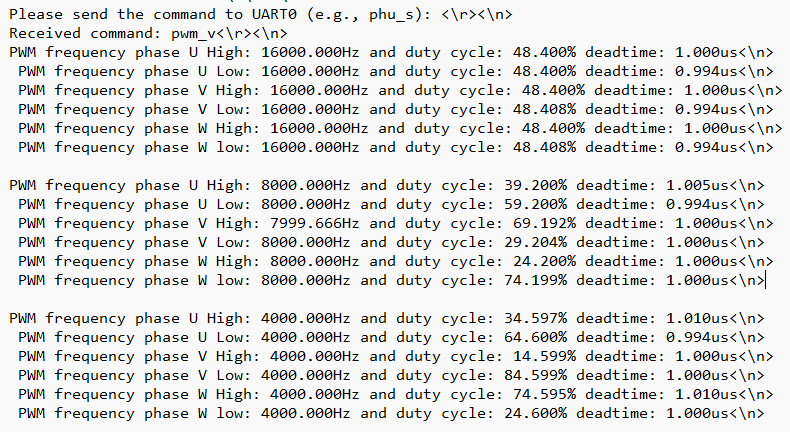
\includegraphics[width=0.90\textwidth]{gfx/diagrams/PWM_Results.png}
	\caption{\acs{PWM} Verification Results}
	\label{fig:Results:PWM_Results}
\end{figure}

The figure displays results from three representative test sequences. In the first sequence, the \acs{PWM} frequency is configured to 16 kHz with a 50\% duty cycle for all phases, and the dead time is set to 1 $\mu$s. In the second sequence, the \acs{PWM} frequency is 8 kHz, and the duty cycles differ by phase (for example, UH/UL at 40\%/60\%, VH/VL at 70\%/30\%, and WH/WL at 30\%/70\%). In the third sequence, the \acs{PWM} frequency is set to 4 kHz and likewise variable phases.

Across all sequences, the measured duty-cycle values exhibit minor, consistent deviations from the intended settings. This outcome is anticipated, as the 1 $\mu$s dead time reduces the available high-pulse width within each \acs{PWM} period. The measured values presented in the figure \ref{fig:Results:PWM_Results} demonstrate this effect and confirm that the verification platform accurately records the \acs{PWM} characteristics.

\vspace{-1.0\baselineskip}
\section{\acs{OVC} Verification Results}

The Control Board outputs a 2-byte value for each static current level configured by the verification MPSOC. These bytes represent over-current event and status information, as detailed in Section \ref{sec:Implementation:OVC_Verification}. The accompanying figure illustrates the system's response in two representative test cases. When the current remains within the \acs{OVC} limits, the Control Board returns "00", signifying the absence of any overcurrent event or status condition.

In the subsequent test, a value of 0x0000 is applied, which falls outside the permissible \acs{OVC} threshold. In this scenario, the Control Board returns "1F". The first byte signifies that the ovc\_event flag is set, while the second byte indicates that all bits in the ovc\_status field are high. This outcome demonstrates that all three phases are experiencing a short-circuit or fault condition. These results confirm that the \acs{OVC} detection functionality on the Control Board operates as intended for out-of-range current inputs.

\begin{figure}[htbp]
	\centering
	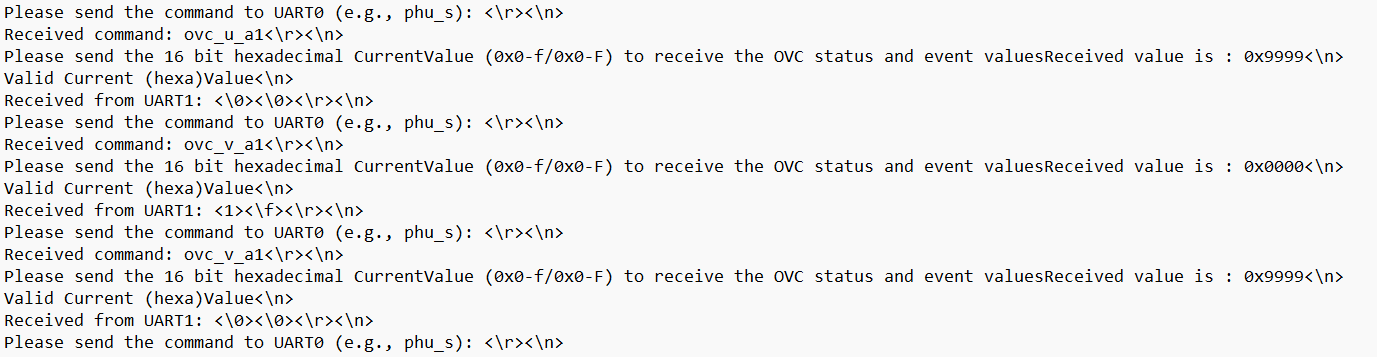
\includegraphics[width=0.90\textwidth, height=0.20\textheight]{gfx/diagrams/OVC_Results.png}
	\caption{Overcurrent module Verification Results}
	\label{fig:Results:OVC_Results}
\end{figure}